\section{Experiment and Analysis}
\label{sec:experiment}

In this section, we introduce the in-field measurements experiments 
, the evaluation of the heterogeneous wireless system 
and analysis of the results.

% Subsec Experiment design
\subsection{In-field Measurements}
\label{subsec:measurements}

We perform in-field measurements in typical areas to find the channel state variation across 
time and the user mobility patterns among the areas.
% 24 hours measurement introduction
We chose neighborhoods, campus, downtown business office and 
urban business office to perform long term 24 hours measurements on weekdays. 
The locations we chosen are located in Downtown Dallas, a university campus in Dallas, 
a business in Dallas urban area and an apartment on north Dallas. 
The locations where we collected measurements are shown in Fig.~\ref{fig:measurement_map}.

\begin{figure}
\vspace{-0.0in}
\centering
\includegraphics[width=84mm]{figures/measurements_map}
\vspace{-0.1in}
\caption{Long Term Measurements Locations}
\label{fig:measurement_map}
\vspace{-0.1in}
\end{figure}

In each of the location, we left our equipment running to measure the channel state for 24 hours during 
weekdays. 
% Experiment equipment
We employ a Rohde \& Schwarz FSH8 portable spectrum works from 100 KHz to 8 GHz. 
The portable spectrum analyzer is controlled by a Python script on a laptop to measure 
the received signal strength.
% Data normalize 
To the best of our knowledge, there is no readily available mobile, multiband antenna from
450 MHz to 5.2 GHz on the market. Thus, we use a 700-MHz mobile antenna to perform in-field
measurements. We then normalize the mobile antenna performance across bands with indoor 
experimentation. To do so, we use a Universal Software Radio Peripheral (USRP) N210 to 
generate signals at 450 MHz, 800 MHz, and 2.4 GHz. We feed the USRP signals directly
to a spectrum analyzer and adjust the configuration of USRP to make the received signal 
strength the same as the 5.2 GHz signal from Gateworks 2358 with a XR5 radio. Then, we connect 
the signal source to a fixed multiband antenna (QT 400 Quad Ridge Horn Antenna) and measure the
received signal at a fixed distance with the 700 MHz antenna and antennas for different bands
to obtain the antenna loss for each band. We adjust the received signal strength
collected via the 700-MHz mobile antenna according to the normalization.
We use $-85 dBm$ as a threshold in the activity level calculation for the normalized data.

% Introduce how to calculate the capacity
% Explain multiband and activity level
When wireless devices operate in WiFi bands, the channel separation is relatively 
small (e.g., 5 MHz for the 2.4 GHz band). As a result, many works assume that
the propagation characteristics across channels are similar. However, with the
large frequency differences between WiFi and white space bands (e.g., multiple GHz),
propagation becomes a key factor in the deployment of wireless networks with both bands.
Here, a frequency band is defined as a group of channels which have
little frequency separation, meaning they have similar propagation characteristics.
In this work, we consider the diverse propagation and activity characteristics
for four total frequency bands: 450 MHz, 800 MHz, 2.4 GHz, and 5.2 GHz.
We refer to the two former frequency bands as white space bands and
the two latter frequency bands as WiFi bands.
The differences in propagation and spectrum utilization create opportunities
for the joint use of white space and WiFi bands in wireless access networks according
to the environmental characteristics (e.g., urban or rural and downtown or residential)
of the deployment location.


Through the measured data set, we calculate the activity level via Eq.~\ref{eq:actdef}.
The activity level is calculated in one minute time window.
We average the activity level in 30 minutes across 24 hours.
% Need to discuss the \mu mapping with these measurements stuff



% FIXME how to show the data
\begin{table*}
\centering % centering table 
\begin{tabular}{|l|c|c|c|c|c|c|c|c|c|c|c|c|c|} % creating 13 columns 
\hline %\hline % inserting double-line 
%Bands     & \multicolumn{3}{c|}{Dallas} & \multicolumn{3}{c|}{Weatherford} & \multicolumn{3}{c|}{Millsap} \\% [0.5ex]
%\hline % inserts single-line 
% Entering 1st row 
%Area Type & Downtown & Residential & Suburban & Downtown &  Residential & Sparse & Downtown & Residential & Sparse \\ % [0.5ex]
%\hline % inserts single-line 
%\multirow{8}{*}{Downtown}	
%&\multirow{2}{*}{Downtown 450 MHz}	
%&0:00-11:00 &  22.09 &  21.27 &  22.28 &  22.47 &  21.65 &  21.68&  22.37 &  22.16&  23.12 &  22.73&  22.01 &  22.54 \\ 	
%\cline{3-15}	
%&&12:00-23:00&  21.80 &  20.86 &  21.80 &  22.54 &  22.35 &  22.61&  22.45 &  21.58&  22.18 &  23.09&  22.11 &  22.09 \\ 	
%\cline{2-15}	
%&\multirow{2}{*}{800 MHz}	
%&0:00-11:00 &  12.99 &  12.44 &  12.08 &  12.32 &  11.60 &  11.60&  12.48 &  12.10&  11.14 &  11.55&  11.98 &  11.12 \\ 	
%\cline{3-15}	
%&&12:00-23:00&  11.88 &  12.27 &  12.36 &  12.05 &  12.15 &  14.00&  13.32 &  12.29&  11.38 &  11.55&  12.92 &  13.16 \\ 	
%\cline{2-15}	
%&\multirow{2}{*}{2.4 GHz}	
%&0:00-11:00 &  29.08 &  29.15 &  29.49 &  28.93 &  29.01 &  28.86&  28.84 &  29.53&  29.03 &  28.74&  29.89 &  29.15 \\ 	
%\cline{3-15}	
%&&12:00-23:00&  28.60 &  29.61 &  29.44 &  28.55 &  28.05 &  28.62&  28.74 &  28.93&  28.26 &  27.73&  28.19 &  29.85 \\ 	
%\cline{2-15}	
%&\multirow{2}{*}{5.2 GHz}	
%&0:00-11:00 &  27.21 &  27.11 &  26.20 &  25.77 &  26.70 &  26.17&  25.67 &  26.10&  25.77 &  25.41&  26.05 &  26.34 \\ 	
%\cline{3-15}	
%&&12:00-23:00&  26.17 &  26.03 &  25.19 &  26.41 &  26.80 &  25.17&  26.08 &  25.60&  26.44 &  26.58&  25.50 &  25.45 \\ 	
%\hline	
%\multirow{8}{*}{Urban}	
%&\multirow{2}{*}{450 MHz}	
%&0:00-11:00 &  23.17 &  23.69 &  23.45 &  22.83 &  23.24 &  23.43&  23.48 &  23.74&  23.69 &  23.36&  23.29 &  23.00 \\ 	
%\cline{3-15}	
%&&12:00-23:00&  22.85 &  22.81 &  23.62 &  23.74 &  23.14 &  23.48&  23.38 &  22.52&  22.04 &  22.59&  22.59 &  22.42 \\ 	
%\cline{2-15}	
%&\multirow{2}{*}{800 MHz}	
%&0:00-11:00 &  12.63 &  13.20 &  13.08 &  12.94 &  11.55 &  11.48&  11.60 &  11.38&  11.86 &  11.72&  10.47 &  10.32 \\ 	
%\cline{3-15}	
%&&12:00-23:00&  12.00 &  11.86 &  10.71 &  11.93 &  12.72 &  12.36&  11.48 &  11.43&  11.72 &  11.60&  11.72 &  11.91 \\ 	
%\cline{2-15}	
%&\multirow{2}{*}{2.4 GHz}	
%&0:00-11:00 &  29.04 &  28.66 &  27.29 &  28.15 &  27.89 &  27.72&  28.18 &  27.38&  28.18 &  27.74&  28.15 &  27.96 \\ 	
%\cline{3-15}	
%&&12:00-23:00&  27.96 &  29.14 &  28.97 &  28.20 &  28.80 &  29.57&  29.02 &  27.72&  27.70 &  27.77&  29.21 &  28.42 \\ 	
%\cline{2-15}	
%&\multirow{2}{*}{5.2 GHz}	
%&0:00-11:00 &  25.41 &  25.29 &  26.32 &  26.49 &  27.23 &  27.28&  26.99 &  26.27&  25.36 &  26.13&  25.81 &  24.88 \\ 	
%\cline{3-15}	
%&&12:00-23:00&  26.92 &  26.49 &  26.41 &  27.11 &  25.67 &  26.53&  26.73 &  26.97&  26.32 &  25.79&  27.57 &  26.65 \\ 	
%\hline	
%\multirow{8}{*}{Campus}	
%&\multirow{2}{*}{Campus 450 MHz}	
%&0:00-11:00 &  20.29 &  21.56 &  21.41 &  22.52 &  23.12 &  21.97&  21.65 &  21.63&  21.87 &  21.22&  21.17 &  21.39 \\ 	
%\cline{3-15}	
%&&12:00-23:00&  22.33 &  22.88 &  22.28 &  21.65 &  22.49 &  22.16&  21.32 &  22.35&  21.56 &  21.75&  21.75 &  20.45 \\ 	
%\cline{2-15}	
%&\multirow{2}{*}{800 MHz}	
%&0:00-11:00 &  11.98 &  12.20 &  12.68 &  12.03 &  11.52 &  11.19&  11.96 &  12.94&  11.52 &  11.93&  12.44 &  10.95 \\ 	
%\cline{3-15}	
%&&12:00-23:00&  11.26 &  11.62 &  12.12 &  12.70 &  12.34 &  11.62&  11.57 &  12.17&  11.55 &  12.08&  11.88 &  11.98 \\ 	
%\cline{2-15}	
%&\multirow{2}{*}{2.4 GHz}	
%&0:00-11:00 &  26.10 &  25.91 &  28.02 &  26.61 &  27.90 &  27.09&  27.01 &  27.21&  26.99 &  26.75&  25.69 &  26.46 \\ 	
%\cline{3-15}	
%&&12:00-23:00&  26.58 &  27.23 &  26.92 &  26.29 &  26.10 &  26.13&  26.25 &  25.53&  25.79 &  25.84&  26.13 &  26.46 \\ 	
%\cline{2-15}	
%&\multirow{2}{*}{5.2 GHz}	
%&0:00-11:00 &  26.68 &  26.05 &  25.12 &  25.93 &  25.36 &  25.79&  26.03 &  26.73&  25.89 &  25.26&  25.81 &  25.50 \\ 	
%\cline{3-15}	
%&&12:00-23:00&  25.19 &  25.60 &  24.52 &  25.00 &  26.08 &  26.17&  26.85 &  26.53&  26.10 &  25.53&  25.89 &  25.31 \\ 	
%\hline	
%\multirow{8}{*}{Neighborhoods}	
%&\multirow{2}{*}{450 MHz}	
%&0:00-11:00 &  23.17 &  24.35 &  23.82 &  23.75 &  23.44 &  22.76&  24.08 &  25.26&  24.54 &  23.87&  23.82 &  23.70 \\ 	
%\cline{3-15}	
%&&12:00-23:00&  23.48 &  22.67 &  23.53 &  23.48 &  23.99 &  24.49&  23.99 &  22.98&  22.86 &  23.03&  23.89 &  23.63 \\ 	
%\cline{2-15}	
%&\multirow{2}{*}{Neighborhoods 800 MHz}	
%&0:00-11:00 &  15.72 &  16.30 &  16.33 &  15.72 &  16.54 &  14.48&  14.62 &  14.48&  15.68 &  15.03&  15.60 &  16.33 \\ 	
%\cline{3-15}	
%&&12:00-23:00&  15.72 &  14.74 &  14.74 &  14.38 &  15.41 &  15.00&  15.84 &  16.25&  14.84 &  14.69&  15.51 &  14.93 \\ 	
%\cline{2-15}	
%&\multirow{2}{*}{2.4 GHz}	
%&0:00-11:00 &  26.49 &  26.37 &  26.22 &  26.03 &  24.97 &  27.16&  27.76 &  26.56&  26.05 &  26.22&  25.74 &  27.18 \\ 	
%\cline{3-15}	
%&&12:00-23:00&  27.01 &  26.34 &  25.79 &  25.48 &  26.53 &  26.29&  25.33 &  25.86&  26.92 &  25.98&  25.48 &  27.66 \\ 	
%\cline{2-15}	
%&\multirow{2}{*}{5.2 GHz}	
%&0:00-11:00 &  25.93 &  26.27 &  25.07 &  25.67 &  26.77 &  26.80&  27.52 &  25.38&  25.55 &  25.86&  25.62 &  26.13 \\ 	
%\cline{3-15}	
%&&12:00-23:00&  25.29 &  26.49 &  26.70 &  26.77 &  25.31 &  24.59&  24.78 &  25.91&  25.67 &  24.73&  24.73 &  25.21 \\ 	

%Subtable here 
\multirow{2}{*}{Downtown 450 MHz}	
&0:00-11:00 &  22.09 &  21.27 &  22.28 &  22.47 &  21.65 &  21.68&  22.37 &  22.16&  23.12 &  22.73&  22.01 &  22.54 \\ 	
\cline{2-14}	
&12:00-23:00&  21.80 &  20.86 &  21.80 &  22.54 &  22.35 &  22.61&  22.45 &  21.58&  22.18 &  23.09&  22.11 &  22.09 \\ 	
\cline{1-14}	
\multirow{2}{*}{Campus 450 MHz}	
&0:00-11:00 &  20.29 &  21.56 &  21.41 &  22.52 &  23.12 &  21.97&  21.65 &  21.63&  21.87 &  21.22&  21.17 &  21.39 \\ 	
\cline{2-14}	
&12:00-23:00&  22.33 &  22.88 &  22.28 &  21.65 &  22.49 &  22.16&  21.32 &  22.35&  21.56 &  21.75&  21.75 &  20.45 \\ 	
\cline{1-14}	
\multirow{2}{*}{Neighborhoods 800 MHz}	
&0:00-11:00 &  15.72 &  16.30 &  16.33 &  15.72 &  16.54 &  14.48&  14.62 &  14.48&  15.68 &  15.03&  15.60 &  16.33 \\ 	
\cline{2-14}	
&12:00-23:00&  15.72 &  14.74 &  14.74 &  14.38 &  15.41 &  15.00&  15.84 &  16.25&  14.84 &  14.69&  15.51 &  14.93 \\ 	
\hline	
\end{tabular}    
\caption{Part of Activity Level in Multiple Locations} % title name of the table 
\label{tab:activitymeasurement}    
\vspace{-0.3in}
\end{table*}    


% Data analysis
% List part of the data
Through the activity level results, we observe that the activities of 450 MHz in the air has almost the same patterns across all 
the four measured areas. The large propagation area of 450 MHz influence the areas simultaneous and the 450 MHz activities are 
perform regularly on weekdays.
Neighborhood area has more activity in 800 MHz than other types of areas. But the 800 MHz activity levels are relatively lower than 
other bands in all the areas.
The WiFi 2.4 GHz channel of neighborhoods has more activity in the night while the downtown area has more activity in the day time.
The campus has more WiFi activities in the morning than the afternoon and night. 
Part of the measurements results are list in Table~\ref{tab:activitymeasurement}.
Due to the limited space, the full list of measurements are available upon request.
We integrate the measurements result into our numerical simulation of GSR algorithm later in this section.




% Mobility pattern measurements
To identify the user mobility pattern, we leverage the data from WiEye database and find the user locations across time.
% WiEye introduction
WiEye application created for the data collection is currently available for download and usage via the Google Android 
Market under the name WiEye. The application offers WiFi access points connection quality in both graphical and tabular 
form. All data collection is done in the background, either continuously while the user is running the application or 
periodically if the user has opted in to background data collection to SMU research. 
The data collected has been approved by the Southern Methodist University Institutional Review Board, a human subjects 
research committee,ensuring that all ethical precautions have been taken in collecting data from the users of our 
application.



% Here, discuss the wieye data process, 
We choose the data from WiEye database according to the GPS location. The data we chosen from
Dallas area, including downtown, urban, SMU campus and neighborhood area. We note the SMU campus 
area size as the unit, find the same size of downtown area and urban area. The rest of the chosen 
locations are counted as neighborhoods. The size of neighborhoods area is about $2.8$ of campus 
area. The data set is generated from Oct. 1st 2014 to March 20th 2015. 
We track the identified 538 users from the data set in different types of areas. 
The number of users located in these area are counted according to the GPS and further converted into 
the percentage each hour. The percentage distribution of users across these areas during a weekday is shown 
in Fig.~\ref{fig:wieyeprocess}

\begin{figure}
\vspace{-0.0in}
\centering
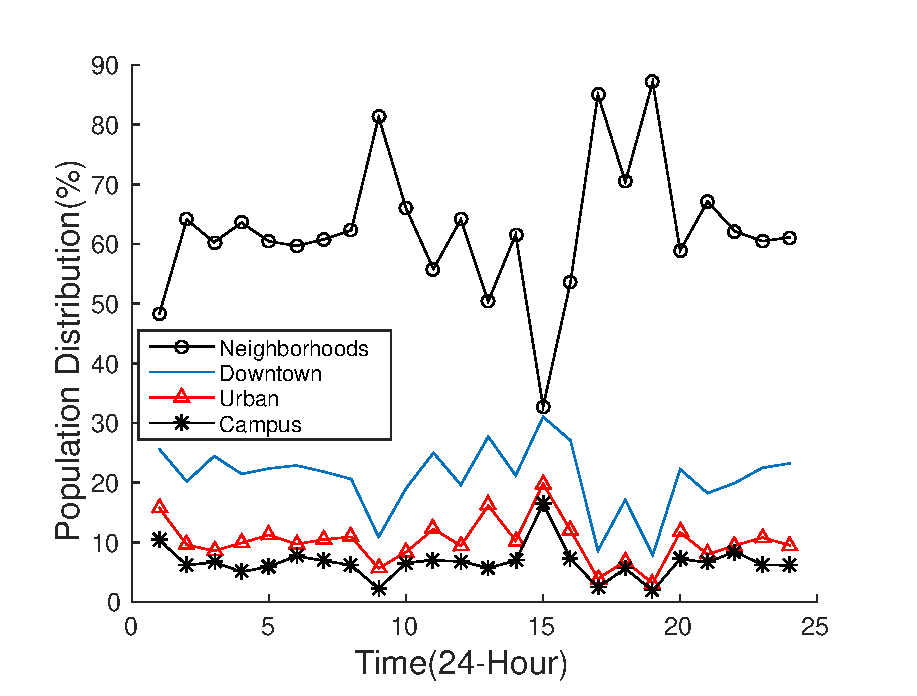
\includegraphics[width=84mm]{figures/wieyeprocess}
\vspace{-0.1in}
\caption{User Distribution across Time}
\label{fig:wieyeprocess}
\vspace{-0.1in}
\end{figure}

From the measurements results, we could find the distribution increase from 9:00 AM in the morning till 
3:00 PM in the afternoon in downtown, urban business area and campus. 
This match the most of the work schedule.
The peak of neighborhoods is around 6:00 PM in the afternoon and 9:00 AM in the morning. 
The reason could be the users are looking for breakfast in the morning before go to work.
We input the user mobility pattern into our power consumption numerical simulation.



\subsection{Experiments, Results and Analysis}
\label{subsec:experimentsetup}

% Virtual city setup
We apply our GSR algorithm with the measurements in a virtual city to investigate white space band 
impacts on power consumption. 
The virtual city in our experiment includes a downtown area, a school campus area, two urban business 
areas and three neighborhood areas. 
All the areas are in the same size with a single WiFi cell. 
The white space channels has more than 3 times propagation range than WiFi channels 
even with the lowest frequency WiFi channel and the highest white space channel.
The white space radios are located in the center of the virtual city cover all the users in the 
four types of areas.
We assume the residents in the city is a constant number which could be calculated through the 
population distribution according to the 2010 U.S. Census~\cite{uscensus}. 
The channel variation of spectrum is setup according to the channel state measurements
and the user mobility from the measurements results of WiEye introduced in 
Subsection~\ref{subsec:measurements}.

% Time population, user traffic demand and radios capacity setup
The transmit power of radios are equal and with the same clean channel capacity. 
The standby power consumption of a radio is 500 watt and transmit power is 1 watt per Mbps.
We lookup population distribution from the US census 2010 to calculate the users in the 
virtual city. We set the demand requested per user as 0.5 Mbps and assume 30\% of the users will 
activate their device (ie. the take rate is 30). The tolerance time of users is $30\ ms$ in most of 
the simulations. We adopt an 802.11n maximum data rate of 600 Mbps for all the radios. 
For the single white space channel setup, the channel is from the 800 MHz. For two white space channels, 
one is 450 MHz, the other one is from 800 MHz. For three white space channels setup, two of them are from 
800 MHz and one from 450 MHz.

% Investigate time
We first investigate the power consumption variation across time with the population distribution 
as $2000 ppl/km^2$ with the measurements setup. The results across 24 hours of the virtual city 
is shown in Fig.~\ref{fig:timevary}

\begin{figure}[hpt]
\vspace{-0.0in}
\centering
\includegraphics[width=84mm]{figures/timevary}
\vspace{-0.1in}
\caption{Power Consumption across Time}
\label{fig:timevary}
\vspace{-0.1in}
\end{figure}

We observe that the WiFi power consumption keeps constant in most case. That because the WiFi 
propagation range restrict all the radios have to be on operating to serve the users. While the 
white space radios could adapt the user non-uniform distribution or user mobility better. When the 
user distribution changes fast at 9:00 AM, the white space configurations could reduce the power 
consumption by about 20\% of the previous user distribution. Three white space channels could 
reduce almost half of the power consumption in the simulation. 
The power consumption gain is mainly from turning off the radios.
% uniform distribution does not have a great gain
When the users are uniform distributed, the power consumption may increase due to the splitting of
white space channels. The queuing theory concludes that a single faster server is better than 
multiple slower server have the same capacity. When the users are uniform like distributed, the 
white space channels may be divided into several sub-channels which lower the performance. 
From the measurements numerical simulation, one white space channel could reduce the power consumption 
by 24.57\% during 24 hours. Two white space channels could reduce by 46.27\% and three white space channels 
could reduce by 67.40\% relatively. 
As the number of white space channel increase, the power consumption gains per channel will become a 
constant since there is enough channel capacity to satisfy the users.
Thus, according to the result, we could design the network with white space channels to adapt the user 
mobility patterns with affordable power consumption as well as apply the 
white space channels as complement resource for the existing WiFi infrastructure.



% Different cities
Further, we study the tolerance waiting time $W$ of users impacts on the power consumption. 
We keep the population distribution as $2000\ ppl/km^2$ and 11:00 AM channel state and 
user distribution.
The tolerance waiting time is set from $5\ ms$  to $90\ ms$ with $5\ ms$ steps. The results 
are shown in Fig.~\ref{fig:delayvary}.
 
% Delay variation
\begin{figure}[hpt]
\vspace{-0.0in}
\centering
\includegraphics[width=84mm]{figures/delay_vary}
\vspace{-0.1in}
\caption{Power Consumption across Delay Tolerance}
\label{fig:delayvary}
\vspace{-0.1in}
\end{figure}

% Fit for long delay tolerance,if small delay require more resource
The results that the less quality of service in waiting time, the less power consumption is required.
As the tolerance waiting time increase, the power consumption of both WiFi and heterogeneous configuration 
gains power saving. The WiFi configuration gains the power saving mainly from the reduction of channel 
capacity delivery. The white space configuration gains the power saving from both the reduction of channel 
capacity delivery and the sleeping radios. Thus, there are some sharp reduction in the white space setup 
in the numerical simulation results due to the radio turning off.
The power consumption could be reduced by 170.24\% with three white space channels under the tolerance waiting 
time $90\ ms$.
When the tolerance waiting time is more than $50\ ms$ there is no great difference between the two white space 
channels setup and three white space channels setup. 
As discussed in previous section, most of the major cities in the U.S. has restriction of white space channels.
Thus, the network carriers is able estimate the quality of service they can offer according to the resource they 
own, such as the number of white space channels, the power supply, etc.



We involve the previous measurement work of channel state in multiple cities in DFW metroplex area to study the 
population density variation in white space network design~\cite{pcuiwinmee}.
We choose the 
The achieved channel capacity is mapping to the population distribution as in~\cite{pcuiwinmee}. The user 
distribution is set as our measurements in 11:00 AM with $30\ ms$ tolerance waiting time.
The results are shown in Fig.~\ref{fig:populationvary}.

% Not sentivitv to population? need more resultes
\begin{figure}[hpt]
\vspace{-0.0in}
\centering
\includegraphics[width=84mm]{figures/populationvary}
\vspace{-0.1in}
\caption{Power Consumption across Population Distribution}
\label{fig:populationvary}
\vspace{-0.1in}
\end{figure}

As the population increase, all the configuration of network cost more power to serve the users.
The gains of a single white space channel reach the peak in 50 $ppl/km^2$ as 512.55\%. 
And the users are able to be satisfied by only one white space channel, the increasing of white space 
channels does not gains in power consumption. The same result happens for 100 $ppl/km^2$ with more than 
two white space channels. The number of white space channels reaches the constant power consumption 
increase with the population. For 50 $ppl/km^2$ is one white space channel while 100 $ppl/km^2$ needs two 
white space channels. Also, the gain of a single white space channels decrease as the number of white space 
channels increase. Such as in 1000 $ppl/km^2$, the first white space channel gains 70\% of power consumption, 
the second channel adding to the system gains only 47.98\% and the third one gains only 2.26\%.  
Thus, when the white space channels are limited, split them into multiple combination of WiFi cells 
could increase the power consumption other than put them in one WiFi virtual city.





% Robust


% Sum
% WiFi fit for constant user set up
We study the white space impacts on the WiFi mesh networks. The application of white space channels reduce the 
power consumption of the system most of the time. The white space channels are good at adapting user mobility 
with less power consumption. Through the numerical simulation, putting the limited white space channels as complementary 
resource for the existing wireless network is able to reduce the power consumption of the system or increase the 
quality of service. When the wireless resource is above a threshold, the gain of white space becomes relatively 
small in the system.


% White space fit for moving users and could be used as supplimanet
